\chapter{Evaluation de la capacité des méthodes développées à assimiler les données sur plusieurs applications}
\newcommand{\xx}{x_0 = 0.02}
\newcommand{\sigx}{\sigma_0^2 = 0.5}
\section{Objectif}

Deux adaptations du filtre EnKF ont été proposées pour permettre l'assimilation de données pour des méthodes sans maillages. En effet, la correction à la Kalman entrainait des solutions dont le nombre de particules augmentait de manière exponentiel. Ainsi les méthodes ont consisté soit à générer une nouvelle distribution de particule (filtre Remesh-EnKF), soit approcher la solution analysée en modifiant les intensités des configurations particulaires de chaque membre (filtre Part-EnKF). Afin de valider ces deux approches, deux études ont été réalisées. La première présente une méthode unidimensionnelle d'un problème d'advection-diffusion. L'objectif est de mieux visialiser les différentes approches et de les comparer à une solution définies par une discrétisation eulérienne. Dans un second temps, les deux filtres sont appliqués à à un problème d'écoulement incompressible bidimensionnel non linéaire, résolu via la méthode Vortex-In-Cell (VIC) pour évaluer qualitativement le comportement des différents filtres.

\section{Problème 1D d'advection diffusion}~\label{sec:App_1D}

Nous définissons un problème de convection-diffusion unidimensionnel $2\pi$-périodique suivant l'équation

\begin{equation*}
    \frac{\partial u}{\partial t}(x,t) + v \frac{\partial u}{\partial x}(x,t) = \visc \frac{\partial^2 u}{\partial x^2}(x,t),
\end{equation*}

avec $x$ la coordonnée spatiale, $v$ une vitesse constante et $\visc$ un coefficient de diffusion constant.
Pour l'application suivante, la solution de référence utilise les paramètres $v = \refv$ et $\visc = \refvisc$.
Nous définissons le noyau de chaleur périodique $2\pi$ en une dimension comme suit

\begin{equation*}
    \phi(u, s) = \sum_{k=-\infty}^{\infty} \frac{1}{\sqrt{4 \pi s}} \exp{\left(-\frac{{(u - 2\pi k)}^2}{4s} \right)}.
\end{equation*}

Considérant une condition initiale caractérisée par une forme gaussienne exprimée comme $u^{gt}(x, 0) = \phi(x-x_0, Dt_0)$, où $\xx$, $t_0 = \frac{\sigma_0^2}{2D}$, et $\sigx$, nous dérivons la solution analytique complète en utilisant la solution de l'équation de Green :

\begin{equation*}
    u^{gt}(x, t) = \phi(x- v t - x_0, \visc (t+t_0)).
\end{equation*}

La solution analytique est alors une fonction gaussienne, caractérisée par une moyenne qui se déplace à la vitesse d'advection et une déviation standard proportionnelle à $t$ et $D$. Cette solution est illustrée dans la Figure~\ref{fig:1d_analytical} à différents pas de temps

\begin{figure}[ht]
    \centering
    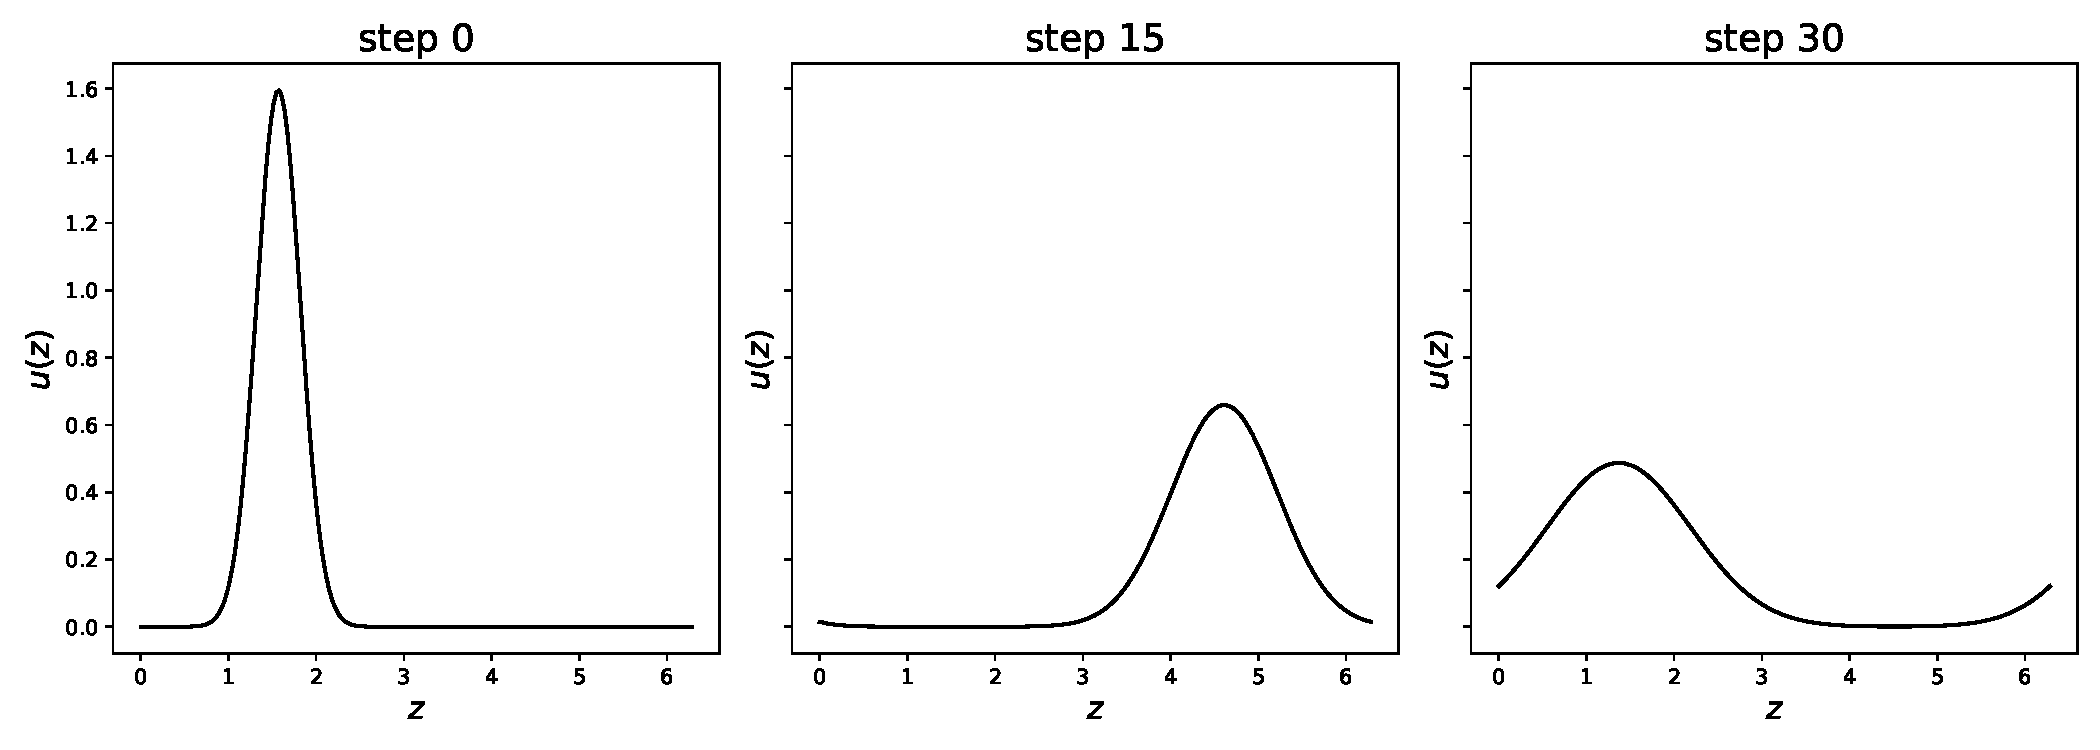
\includegraphics[width=\linewidth]{images/app1d/analytical_frame.pdf}
    \caption{La solution analytique du problème de convection-diffusion évolue au fil du temps.}
    \label{fig:1d_analytical}
\end{figure}

La forme lagrangienne des équations s'écrit

\begin{equation*}
    \frac{dx_p}{dt} = v(x_p, t), \quad \frac{dU_p}{dt} = D \frac{d^2 U_p}{dx^2}
\end{equation*}

Tout comme la méthode vortex décrite en Section~\ref{sec:vortex}, la résolution est réalisée en appliquant un schéma en deux étapes (\textit{viscous splitting}). où l'advection est réalisée au travers d'un schéma d'intégration euler explicite et l'opérateur laplacien est approché en toute position $\bx_p$ comme

\begin{equation*}
    \frac{dU_p}{dt} = D \varepsilon^{-d} V_p \sum_q (U_q - U_p) \phi_\varepsilon( x_q -  x_p),
\end{equation*}

% à mettre partie VIC
Le problème étant périodiques décrit dans la section \ref{App_1D}, nous définissons une fonction noyau équivalente $\phi_\varepsilon= \phi^P_g = \sum_{n=-\infty}^{+\infty} \phi_g(r - 2 \pi n)$.

Le modèle basé sur les particules utilise une discrétisation de \npart{} particules avec une taille de $h = \frac{L}{N_{\text{part}}}$ et une longueur de lissage de $\varepsilon = 1.3 h$.
Pour des raisons de comparaison, nous résolvons l'équation de convection-diffusion avec un schéma explicite de différences finies centrales discrétisé sur une grille régulière avec \ngrid{} nœuds.
\section{Bilan}